%%%%%%%%%%%%%%%%%%%%%%%%%%%%%%%%%%%%%%%%%%%%%%%%%%%%%%%%%%%%%%%%%%%%%%%%%%%%%%%%
\subsubsection{2.5D Experiments}\label{subsubsec:singl_img_2d_lk_experiments}
%%%%%%%%%%%%%%%%%%%%%%%%%%%%%%%%%%%%%%%%%%%%%%%%%%%%%%%%%%%%%%%%%%%%%%%%%%%%%%%%
Our experimental evaluation for 2.5D input data is split into two parts: using
normals as features for Affine Lucas-Kanade parametric image alignment and
using the KPCA framework to construct normal AAMs. In contrast to
\citet{antonakos2015feature}, we choose to compute our features \textit{after}
image warping in order to ensure that the normals we are computing are still
valid normals that exist on the surface of the unit sphere. Therefore, in all
cases we warp the depth values and then compute the normals after the
warping.

\textbf{Affine Lucas-Kanade Experiments.} In these experiments we use data
from the Bosphorus~\cite{Savran:2008gg} database which provides depth images
of 105 subjects under various expressions and occlusions. Given the pre-cropped
nature of these input images we do not perform any pre-processing on the
images other than a similarity alignment between the eye and mouth landmarks to
ensure that the input images all have the same size. We also centre the depth
values to mitigate any scaling issues. In all experiments we used the 
Inverse Compositional algorithm with an Affine motion model.
We defined the template to be a padded
bounding box around the salient regions of the faces, namely the eyes, nose and
mouth. An example template is given in \cref{fig:single_img_2d_lk_examples}.
The Bosphorus dataset is particularly interesting as it contains a number of
images displaying occlusions. This allows us to empirically verify our assumption
that normals represent a more robust feature descriptor than depth values alone.
An example occluded image is given in
\cref{subfig:singl_img_depth_2d_lk_template_occluded}.

We compare the performance of our proposed IP and SPHERICAL features against
depth data alone for the first 5 subjects of the database. The neutral frame
for each subject is chosen as the template and 10 random affine perturbations
of this initial bounding box ($\sigma = 0.04$) are generated for each image 
of a given subject.
\cref{fig:single_img_2d_lk_results} shows the results of this experiment in
the form of a cumulative error distribution (CED) graph which presents
the euclidean error of the bounding box corners normalised by the
average edge length of the ground truth bounding box.
\cref{subfig:singl_img_depth_lk_results_all} shows the cumulative results for
all of the considered subjects. Here we note that both of our proposed
feature descriptors outperform depth data by a comfortable margin. However,
to further demonstrate the effect of the normal descriptors in the case of
occlusions we provide \cref{subfig:singl_img_depth_lk_results_dirty} which
shows the results on the subset of images containing occlusions. Note that
the performance of the depth alignment is significantly degraded by presence
of occlusions in the target image. In contrast, our proposed normal descriptors
provide strong alignment characteristics even in the presence of these
severe occlusions.
%%%%%%%%%%%%%%%%%%%%%%%%%%%%%%%%%%%%%%%%
\begin{figure}[t]
    \centering
    \hspace*{\fill}
    \begin{subfigure}[b]{0.2\textwidth}
    	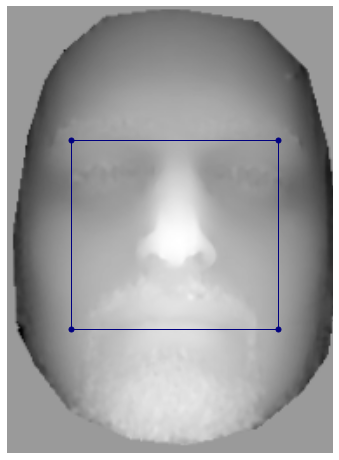
\includegraphics[width=\textwidth]{statistical_normals/images/lk2d/bs004_template.png}
    	\caption{Template}\label{subfig:singl_img_depth_2d_lk_template}
    \end{subfigure} \hfill
    \begin{subfigure}[b]{0.2\textwidth}
    	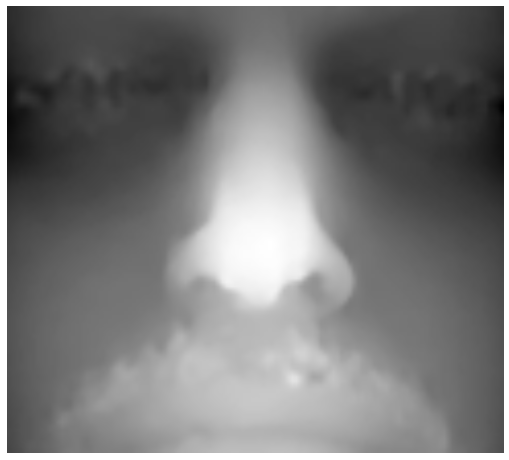
\includegraphics[width=\textwidth]{statistical_normals/images/lk2d/bs004_template_cropped.png}
    	\caption{Template Cropped}\label{subfig:singl_img_depth_2d_lk_template_cropped}
    \end{subfigure} \hfill
    \begin{subfigure}[b]{0.2\textwidth}
    	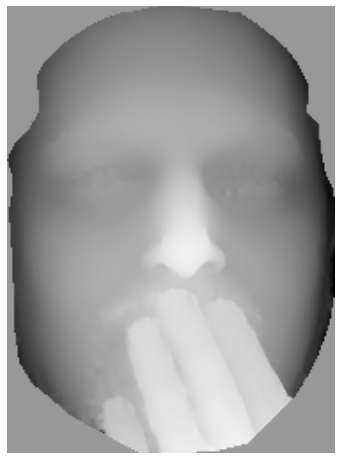
\includegraphics[width=\textwidth]{statistical_normals/images/lk2d/bs004_occluded.png}
    	\caption{Occluded}\label{subfig:singl_img_depth_2d_lk_template_occluded}
    \end{subfigure}
    \hspace*{\fill}
    \caption{An example template from the LK experiments.
             \cref{subfig:singl_img_depth_2d_lk_template_occluded} shows an
             example of an occluded image.}
\label{fig:single_img_2d_lk_examples}
\end{figure}
%%%%%%%%%%%%%%%%%%%%%%%%%%%%%%%%%%%%%%%%
%%%%%%%%%%%%%%%%%%%%%%%%%%%%%%%%%%%%%%%%
\begin{figure}[t]
    \centering
    \hspace*{\fill}
    \begin{subfigure}[b]{0.49\textwidth}
    	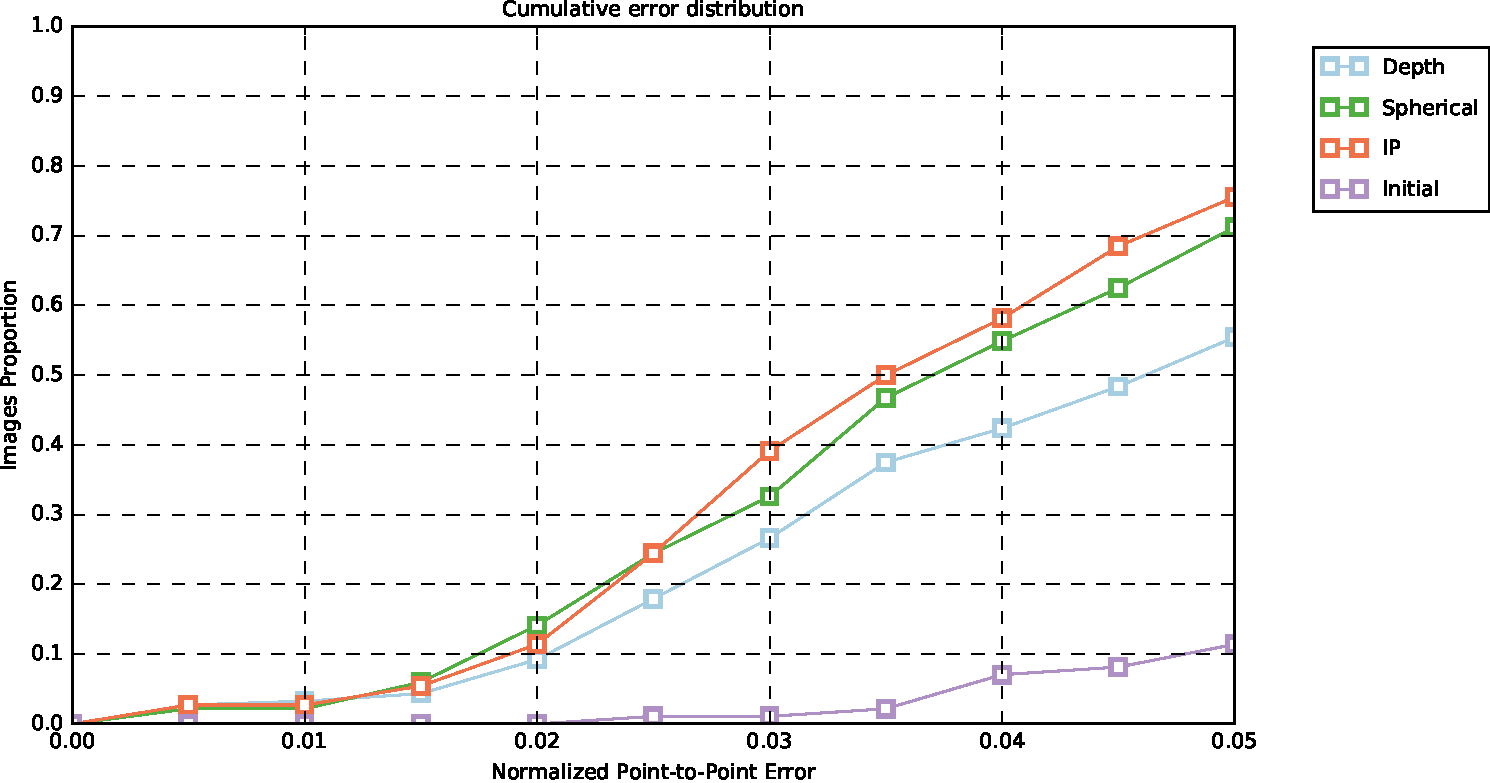
\includegraphics[width=\textwidth]{statistical_normals/images/lk2d/lk_first_5_bosphorus}
    	\caption{All}\label{subfig:singl_img_depth_lk_results_all}
    \end{subfigure} \hfill
    \begin{subfigure}[b]{0.49\textwidth}
    	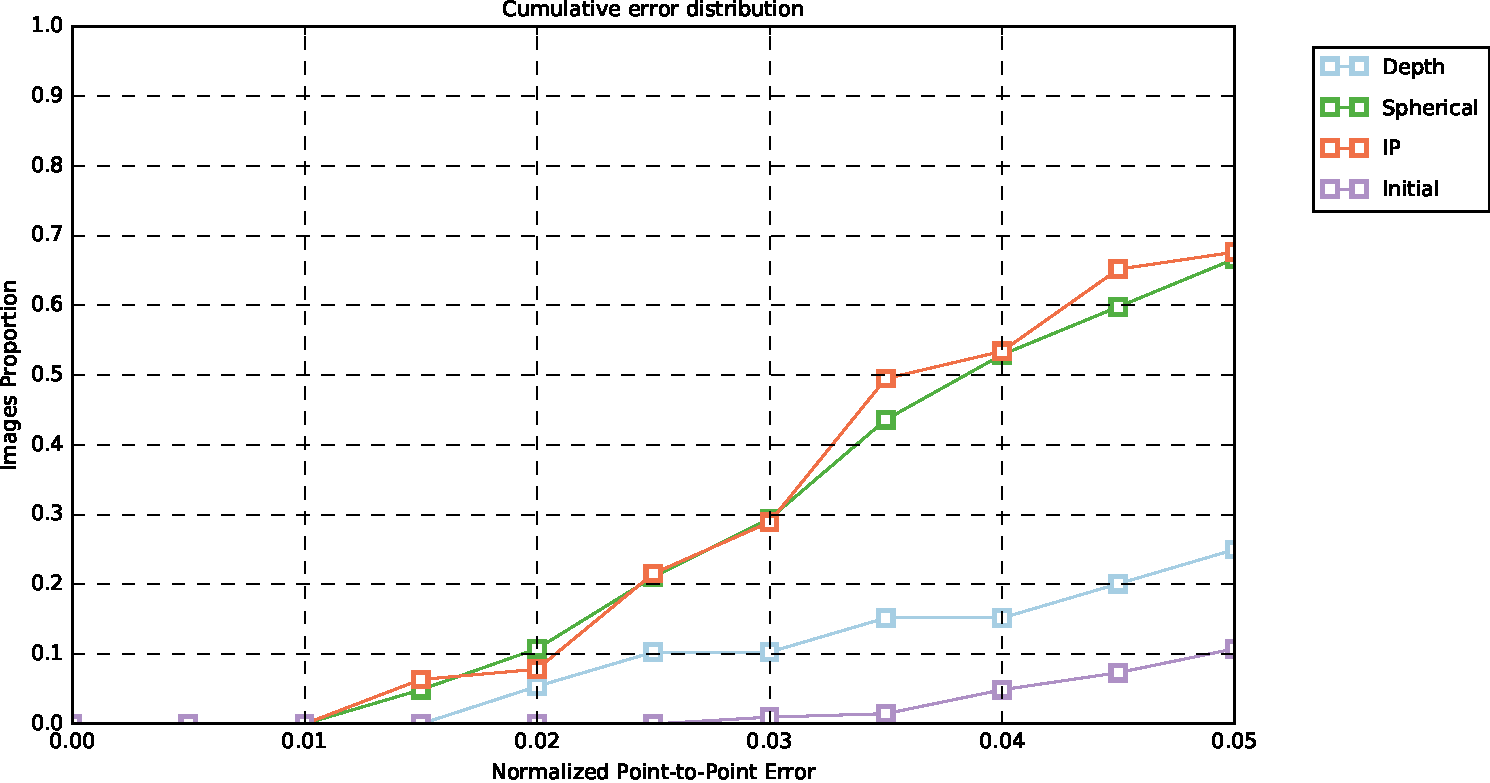
\includegraphics[width=\textwidth]{statistical_normals/images/lk2d/lk_first_5_bosphorus_dirty}
    	\caption{Occluded Only}\label{subfig:singl_img_depth_lk_results_dirty}
    \end{subfigure}
    \hspace*{\fill}
    \caption{Results for the Affine LK algorithms on the 
             Bosphorus~\cite{Savran:2008gg} dataset. Results are shown for the
             first 5 subjects from the database for both the uncorrupted images 
             and images containing occlusions.}
\label{fig:single_img_2d_lk_results}
\end{figure}
%%%%%%%%%%%%%%%%%%%%%%%%%%%%%%%%%%%%%%%%

\textbf{AAM Experiments.} In these experiments we assessed the performance
of our AAM models where the appearance models were constructed using the KPCA
kernels described in \cref{subsubsec:singl_img_ca_kpca}. We used images from
the FRGC v2~\cite{phillips2005overview} dataset and the 68-point landmark
annotations provided by \citet{sagonas2013semi}. We split the data into
a training set and a testing set to ensure that our appearance models
were capable of generalising to unseen individuals. Our training set, used
for construction of both the statistical shape model of 68 points and the
appearance models was constructed using a random sampling of 1000 images
from the Spring 2003 subset. Our testing set consisted of 500 images from the
Spring 2004 subset whereby no individuals present in the Spring 2003 training
set were included. The data from the FRGC dataset is very noisy and therefore
to improve the performance of the depth model we performed simple pre-processing.
We applied a $5\times5$ median filter on the depth channel followed by
the Navier-Stokes based inpainting algorithm~\cite{bertalmio2001navier} provided
by OpenCV~\cite{opencv_library}.

For optimising we employed the alternating inverse
compositional algorithm described in \cref{subsec:aam-alternating} and used a
coarse-to-fine fitting strategy consisting of 2-levels with approximate
reference frame diagonals of 75 and 150 pixels. We truncated our statistical
shape model components to 3 and 6 components respectively due to the lack
of out-of-plane rotation present in the dataset. For our appearance models
we truncated the models to 95\% of the appearance variation for each resolution.
\cref{fig:single_img_2d_aam_means} shows examples of the appearance model
means for the 3 appearance model subspaces considered here: depth, IP and
SPHERICAL. \cref{fig:single_img_aam_results} shows the results of our
experiment in the form of a CED graph showing the mean euclidean error
per point normalised by the average edge length of the ground truth
bounding box. For initialisation we generated random perturbations of the
ground truth bounding box using the parameters of a similarity transformation
$\sigma = 0.04$. Note that our proposed normal kernels outperform the depth
features by a large margin, despite the pre-processing applied to the input
data. In fact, \cref{fig:single_img_2d_aam_examples} shows some examples
of the fitting results for the considered kernels. Note that the depth model
is unable to successfully align the input images when the initialisation is
very challenging as is the case in the first row.
%%%%%%%%%%%%%%%%%%%%%%%%%%%%%%%%%%%%%%%%
\begin{figure}[t]
    \centering
    \hspace*{\fill}
    \begin{subfigure}[b]{0.25\textwidth}
        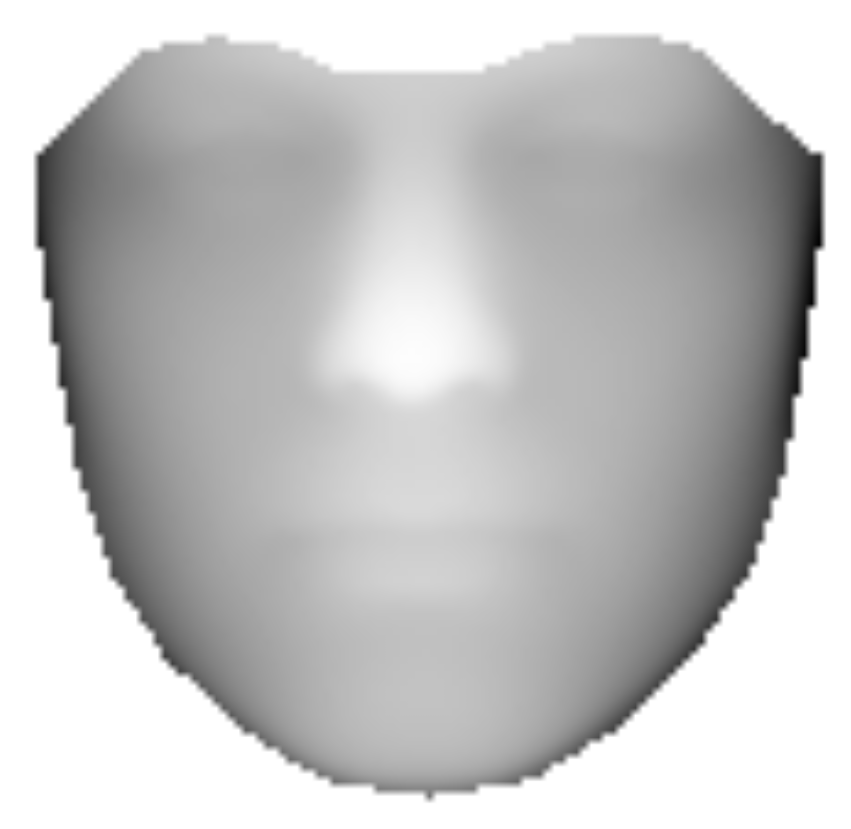
\includegraphics[width=\textwidth]{statistical_normals/images/lk2d/depth_aam_mean.png}
        \caption{Depth Mean}\label{subfig:singl_img_depth_aam_mean}
    \end{subfigure} \hfill
    \begin{subfigure}[b]{0.4\textwidth}
        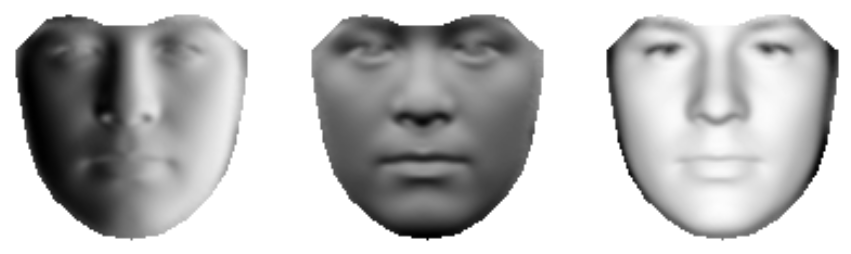
\includegraphics[width=\textwidth]{statistical_normals/images/lk2d/normals_aam_mean.png}
        \caption{IP Mean}\label{subfig:singl_img_ip_aam_mean}
    \end{subfigure} \hfill
    \begin{subfigure}[b]{0.25\textwidth}
        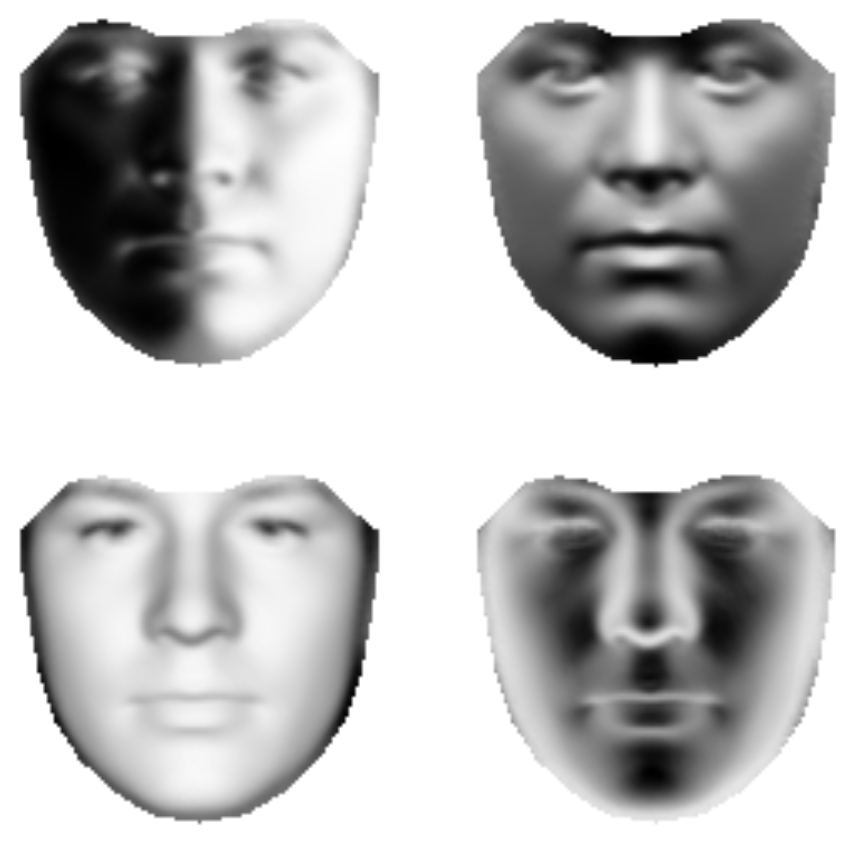
\includegraphics[width=\textwidth]{statistical_normals/images/lk2d/spherical_aam_mean.png}
        \caption{SPHERICAL Mean}\label{subfig:singl_img_spherical_aam_mean}
    \end{subfigure}
    \hspace*{\fill}
    \caption{The appearance model means for the Depth, IP and SPHERICAL 
             AAM models.}
\label{fig:single_img_2d_aam_means}
\end{figure}
%%%%%%%%%%%%%%%%%%%%%%%%%%%%%%%%%%%%%%%%
%%%%%%%%%%%%%%%%%%%%%%%%%%%%%%%%%%%%%%%%
\begin{figure}[t]
    \centering
    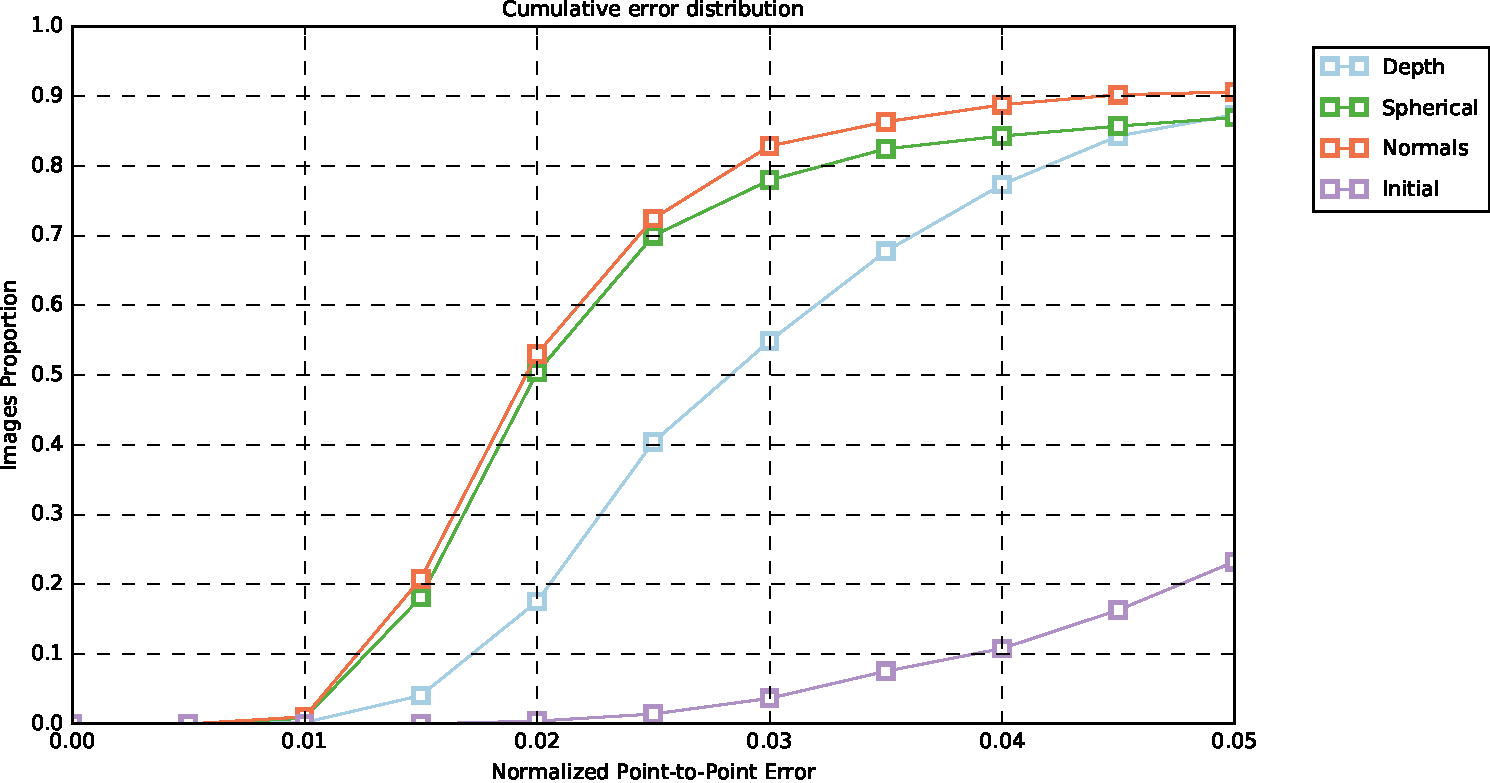
\includegraphics[width=0.7\textwidth]{statistical_normals/images/lk2d/aam_fgrc_500_random}
    \caption{Cumulative Error Distribution (CED) graph for fitting the AAM
             models on 500 random samples from the Spring 2004 subset of the
             FRGC v2~\cite{phillips2005overview} data. The models were trained
             using 1000 random images from the Spring 2003 subset with no
             overlapping identities between the training and testing data.}
\label{fig:single_img_aam_results}
\end{figure}
%%%%%%%%%%%%%%%%%%%%%%%%%%%%%%%%%%%%%%%%
%%%%%%%%%%%%%%%%%%%%%%%%%%%%%%%%%%%%%%%%
\newcommand{\aamrow}[1]{%
\adjustbox{valign=m,vspace=1pt}{\includegraphics[width=3.3cm]{statistical_normals/images/lk2d/#1_gt}}        &
\adjustbox{valign=m,vspace=1pt}{\includegraphics[width=3.3cm]{statistical_normals/images/lk2d/#1_initial}}   &
\adjustbox{valign=m,vspace=1pt}{\includegraphics[width=3.3cm]{statistical_normals/images/lk2d/#1_depth}}     &
\adjustbox{valign=m,vspace=1pt}{\includegraphics[width=3.3cm]{statistical_normals/images/lk2d/#1_ip}}        &
\adjustbox{valign=m,vspace=1pt}{\includegraphics[width=3.3cm]{statistical_normals/images/lk2d/#1_spherical}}
}

\setlength{\tabcolsep}{1pt}
\begin{figure}[t]
    \centering
    \begin{tabular}{ccccc}
        Ground Truth & Initial & Depth & IP & SPHERICAL \\ \vspace{-0.3cm}
        \aamrow{04689d98}                               \\ \vspace{-0.3cm}
        \aamrow{04708d163}
    \end{tabular}
    \caption{Examples of fitting the AAM models on the 
             FRGC v2~\cite{phillips2005overview} data. The first row shows an
             example of a failure by the depth model due to the challenging
             initialisation. The second row shows a success for the depth model
             for a simpler initialisation. Note that our normal model was
             successful in both cases.}
\label{fig:single_img_2d_aam_examples}
\end{figure}
\setlength{\tabcolsep}{6pt}
%%%%%%%%%%%%%%%%%%%%%%%%%%%%%%%%%%%%%%%%
